\documentclass{amsart}
\title[Simulating indirect reciprocity using PageRank]{Simulating
  Evolution of Indirect Reciprocity with Reputation using PageRank}  
\author{Arpon Raksit \and Ben Kuhn \and Rahul Dalal}
\date{\today}
\usepackage{enumitem,graphicx}
%\usepackage[margin=1.75in]{geometry}

\newcommand{\lf}{\left}
\newcommand{\ri}{\right}
\newcommand{\eps}{\epsilon}
\newcommand{\om}{\omega}
\hyphenation{PageRank}

\begin{document}

\begin{abstract}
A key question in the study of evolutionary dynamics has been how
indirect reciprocity might emerge: that is, how individuals might
evolve a tendency to accept a personal fitness cost in exchange for a
greater benefit to another individual, without the understanding that
the recipient will later repay them. One proposed mechanism for this
to occur is that donating to others enhances one's reputation, making
third parties more likely to donate to the donator. We develop a novel
model for determining reputation, adapted from the PageRank Web search
algorithm, that allows individuals to differentiate between refusal to
donate because the donor is selfish, and refusing to donate because
the recipient is selfish. Thus donors will be penalized less for being
paired against a number of selfish individuals. Using this model, we
find that cooperation can emerge with much smaller benefit/cost ratios
than previously observed.
\end{abstract}

\maketitle

\section{Introduction}

In studying the evolutionary origins of altruistic behavior, one of
the most common mechanisms considered is that of reciprocity: an
individual accepts a cost to itself in order to grant a greater
benefit to another. In the most intuitive versions of reciprocity, the
payback (in the form of a reciprocal donation) is immediate; that is,
the players are playing some iterated game where non-cooperation can
immediately be punished. However, ``in the wild'' we often observe
even more altruistic behavior, in which an individual sacrifices some
fitness even when it is not guaranteed that the beneficiary will ever
have the ability to reciprocate, under the assumption that other
members of the population will do a similar service to the donor. This
type of interaction is termed ``indirect reciprocity'' and there are
several proposed mechanisms for it.

We consider the mechanism of reputation: when an individual chooses to
donate, it enhances their reputation in the population, and
individuals are more likely to donate to individuals with higher
reputation. Reputation models sometimes suffer from several
problems. In many models, individuals are penalized equally for being
selfish no matter the reputation of their opponent, so that if an
otherwise generous player has the bad luck to be paired against
several sociopaths, their reputation will be penalized unfairly. Also,
Leimar and Hammerstein \cite{leimar_evolution_2001} argue that in many
reputational models, the dominant strategy is to consider only one's
own reputation and not the recipients, and allowing these strategies
threatens the evolutionary stability of cooperative ones. We try to
find a model that limits these effects.

In this paper, we adapt the PageRank algorithm from Web searching to
give a reputation score to each individual based on the matrix of
pairwise opinions of each individual about each other. These opinions
are based on the most recent interaction between the two. We give a
stochastic model for the evolutionary dynamics of a population
undergoing reputation interactions and give some arguments as to why
this model is realistic and avoids the problems mentioned above.
%TODO

Using this model, we show that indirect reciprocity can emerge in
large populations with a much lower benefit/cost ratio than previously
shown. We show that altruism can spontaneously emerge and fixate even
in large populations of reasonably selfish individuals.
%TODO based on experimental results

The remainder of the paper is as follows: in section
\ref{sec:related}, we go over previous work and explain our novel
contributions. In section \ref{sec:model}, we describe our model and
explain our parameter choices. In section \ref{sec:results}, we
describe and analyze the results of our simulations. Finally, in
section \ref{sec:conclusion} we draw conclusions and suggest further
areas of research.

\section{Related Work}\label{sec:related}

An initial model of indirect reciprocity was suggested by Boyd and
Richerson \cite{boyd_evolution_1989}. In this model, individuals are
arranged in a ring and each individual picks the strategy ``all
defect'', ``upstream tit-for-tat'' (donate unless your potential donor
is selfish) or ``downstream tit-for-tat'' (donate unless your
recipient is selfish). In this model, Boyd and Richerson found that
reciprocal strategies require relatively high concentrations before
they are evolutionarily favored. They also found that downstream
tit-for-tat was generally much more successful than upstream
tit-for-tat, suggesting that strategies based on the recipient's
reputation are more favorable evolutionarily and indicating that
reputation-based systems may be worthy of consideration.

Nowak and Sigmund have modeled indirect reciprocity with a concept of
``image'' \cite{nowak_evolution_1998}. Each individual in the
simulation is given an image score. During each round of a stochastic
simulation, individuals play a number of single-round donor-receiver
games with other members of the population and have the opportunity to
be either altruistic or selfish; the former increases the image score
and the latter decreases it. Individuals’ strategies are to donate if
the recipient’s image score is above some threshold, but keep the
reward otherwise.

Under these circumstances, Nowak and Sigmund found that in the
simplest model, without mutation, whether cooperation evolves is
determined by the initial fraction of defectors. Adding mutation
causes the population to cycle between discriminating cooperation,
unconditional cooperation, and defection in all cases. Limiting the
number of interactions known by each player makes it difficult to
establish cooperation in large populations. Finally, if players are
conscious of their own reputation and act to increase it when it is
low, cooperation evolves much more easily.

This model is simple and elegant, but it has a few drawbacks. For
instance, it discretizes reputation, which may lead to strange edge
effects. Furthermore, it penalizes equally an individual who defects
because they are playing against a low-reputation opponent, and one
who defects for selfish reasons. Finally, Leimar and Hammerstein
\cite{leimar_evolution_2001} argue that in this model the
evolutionarily dominant strategy is to consider only one's own
reputation and not the recipients, and allowing these strategies
threatens the evolutionary stability of cooperative ones.

One can compensate for the latter two problems by considering not just
``first-order'' strategies (that only depend on the donor's actions)
but also second-order strategies (depending on the recipient's current
reputation) and third-order (depending on the donor's current
reputation).  Using a simpler model, in which individuals are rated on
a binary scale of either ``good'' or ``bad,'' Ohtsuki and Ikawa
\cite{ohtsuki_how_2004} showed that out of all 4,096 third-order
strategies, there are a ``leading eight'' that are significantly more
evolutionarily stable than any others, and all of these take into
account that defection against bad actors should not be penalized.

In our model, as in Ohtsuki and Ikawa's ``leading eight,'' players are
not penalized for refusing to donate to selfish recipients.
Furthermore, we allow for a richer scale of reputation than a binary
good/bad rating, and our model can be extended in many ways to take
into account more complex behavior.

\section{Our model}
\label{sec:model}

\subsection{Parameters}

The basic model comprises a series of rounds in which a number of
donor-receiver games are played. We use the following parameters:

\begin{itemize}
\item $N$ is the size of the population to be tested.
\item $I$ is the number of donor-receiver interactions per round.
\item $b$ is the benefit-cost ratio (fitness benefit to recipient over
  cost to donor).
\item $\omega$ is the selection coefficient (magnitude of cost to
  donor).
\item $\mu$ is the strategy mutation probability.
\item $c$ is the fraction of players that are unconditional.
  cooperators
\item $d$ is the fraction that are unconditional defectors.
\end{itemize}

\subsection{State}

Our model has the following state variables:

\begin{itemize}
\item $M \in \mathcal{M}_N(\{0,1\})$ is an $N \times N$ matrix
  representing the opinions each individual has of the others;
  $M_{ij}$ is 1 if player $i$ donated to $j$ the last time they had
  the chance and 0 if $i$ was selfish. Initially, $M$ is the zero
  matrix.
\item $f \in [0, \infty)^N$ is a vector of fitnesses in the current
  round; at the end of the round, individuals reproduce with
  probability proportional to their fitness.
\item $r \in [0,1]^N$ is a vector of reputations of individuals.
\item $s \in [0,1]^N$ is a vector of strategies; player $i$ will
  donate to any player $j$ with $r_j > s_i$ and keep the reward
  against other players.
\end{itemize}

\subsection{Round protocol}
The simulation is initialized by giving each player a random strategy:
unconditional cooperation with probability $c$, unconditional
defection with probability $d$, and a uniform $s \in [0,1]$ with
probability $1 - c- d$. $M$ is originally set to be $0$.

Each round comprises the following steps:

\begin{enumerate}
\item Set all $f_i$ to 1.
\item Compute $r_i$ according to the PageRank algorithm (see below).
\item Determine the results of $I$ interactions (see below).
\item Set entries of $f$ according to the results of the interactions.
\item Set entries of $M$ according to the results of the interactions.
\item Choose a player to die at random and one to reproduce
  proportional to fitness. Replace the dead player with a copy of the
  reproducing one (inheriting the appropriate row and column of $M$,
  but ensuring that the diagonal is always set to 0).
\item With probability $\mu$, the strategy of the new player resets
  randomly as in the initialization phase.
\end{enumerate}

\subsection{PageRank}
\newcommand{\tM}{\tilde M} We think of the matrix $M$ as a directed
graph with some $M_{ij} = 1$ representing an edge from $j$ to $i$---in
other words $j$ has endorsed $i$. Noting an analogy between these
endorsements and links between web pages, we run the standard PageRank
algorithm \cite{page_pagerank_1999} on this graph. (See section
\ref{sec:whypagerank} for an explanation of why this is a realistic
algorithm for individuals to employ.)

Given a matrix $M$, we compute the PageRank as follows. Let $\tM$ be
the column-normalization of $M$, so that $\tM_i = M_i / \sum_j
M_{ij}$. (We need a column-normalized matrix to run PageRank, since it
is based on interpreting the matrix as a Markov chain). The idea of
PageRank is to treat $\tM$ as a Markov chain and find its stationary
probability. The Perron-Frobenius theorem says that $\tM$ has a unique
non-negative eigenvector (and therefore a unique PageRank vector) if
and only if it is irreducible. But we are not necessarily guaranteed
that this is the case: there easily may be a player who has not been
cooperated with. Therefore, we add some ``teleportation probability''
$\alpha$ such that from any given state there is a probability
$1-\alpha$ of going to a random state.

We compute PageRank using the iterated multiplication method; that is,
let $u$ be a uniform vector, $r_0 = u$, and let $r_i =
(1-\alpha)\tilde M r_{i-1} + \alpha u$. Once the difference between
successive $r_i$ is small enough, the last computed vector is the
PageRank.

We make one modification to the PageRank algorithm. Because $r$ is
normalized to the sum of the entries being $1$, this algorithm does
not discriminate between the entire population cooperating and the
entire population defecting. Therefore, at the end we multiply $r$ by
$C/(N-1)$, where $C = \sum_{i,j} M_{ij}$ is the sum of the entries in
the opinion matrix (a measure of how cooperative the current
population is). Note that $0 \le C \le N(N-1)$, the lower bound
occurring if all players are defecting and the upper bound if all
players are cooperating. Hence the maximum of each $r_i$ is $1$.

\subsection{Interaction protocol}
In each round $I$ ordered pairs $(i,j)$ of distinct players are
chosen, each pair independent of the others (note that this means that
in a given round, the same pair can be chosen more than once). Each
$i$ has a choice to decrease its own fitness by $\omega$ to increase
the fitness of $j$ by $b \omega$. The choice is made according to the
strategy of player $i$: cooperation occurs if and only if $s_i <
r_j$. If cooperation occurs, $M_{ij}$ is set to 1, otherwise
$M_{ij}$ is set to $0$.

\subsection{Modifications}
We tested a few modifications of the original model
\begin{enumerate}
%please add or remove as necessary
\item
There is a small probability $\alpha$ that a player does the opposite
of what it wants to in an interaction
\item
There is a small probability $\beta$ that after a donation, the
corresponding entry of $M$ is not updated.
\item
When an individual reproduces, all players' opinions of the offspring
are set to 0.
\item
Each player computes a different number of steps $n_i$ of the PageRank
iterated multiplication representing different capacities for analysis
of social situations. For example, someone who just does $1$ step
would measure reputation as the total number of donations a player
gave replicating Nowak and Sigmund's original model. The $n_i$ are
initialized randomly, are inherited, and mutate with some probability
$\mu_n$. There is a fitness cost $p n_i$ to each player $i$,
reflecting the evolutionary disadvantage from devoting more resources
to social computation.
\item
When an $M_{ij}$ entry is updated a weighted average with some weight
$m$ is taken with the new value and the old value representing some
memory of past interactions.
\end{enumerate}

\section{Analysis of model}
\label{sec:analysis}
\subsection{Donation Game}
As with the model of Nowak and Sigmund, we use the one-shot donation game to remove all effects of direct reciprocity and focus only on the indirect. 

\subsection{Use of PageRank}
\label{sec:whypagerank}

The PageRank algorithm is frequently used to calculate reputation in
social networks \cite{pujol_extracting_2002}. There are a few features
of PageRank that make it desirable for our simulation:
\begin{enumerate}
\item
The opinions of more generous players matter more. This is because
more generous players have more endorsements pointing to them, and
thus better reputation; therefore an endorsement from a high-raking
individual confers more reputation on the receiver than a reputation
from a lower individual. For this reason, optimal strategies must take
into account the receiver's reputation as well as the donor's,
resolving Leimar and Hammerstein's complaint
\cite{leimar_evolution_2001} that reputation dynamics do not properly
incentivize players.
\item
Conversely, the effects of selfishness against low-ranked individuals
are minimized: low-reputation groups cannot unilaterally affect the
PageRank graph by a large margin
\cite{langville_deeper_2004}. Therefore, as mentioned above, generous
individuals will not be unduly penalized for encountering a number of
selfish individuals and refusing to cooperate.
\end{enumerate}

\subsection{Interactions per round}
\label{sec:inter_per_round}

While it is customary to have every member of the population interact
every round of the simulation, we chose instead to pick random pairs
of members interact. This is because if two players are assured of
encountering each other again in the future, the opinion
matrix/PageRank system could essentially act as a proxy for a direct
reciprocity calculation. To make sure that this effect was mitigated,
we chose values for $I$ that ensured the two interacting organisms
were not likely to encounter one another again before they died.

Specifically, in a population of $N$, since one player dies every
round, each player dies with probability $1/N$ and so a player's
lifespan is a geometrically distributed random variable with mean
$N$. If we pick $I=N$, then on any given round and for any given
players $A$ and $B$, player $A$ interacts with $B$ with probability
$1/N$. Therefore if $I\le N$ we expect on average one interaction
between any two given players before one dies. This should be enough
to minimize the effects of our model proxying direct reciprocity.

\section{Results}
\label{sec:results}

\subsection{Dependence on iterations per round}

For each of the population sizes $N \in \{10,20,50,100\}$, increasing
the number of iterations per round increases the probability that
cooperation will fixate, as shown in figures
\ref{fig:pop10iter}--\ref{fig:pop100iter} (with $b=5, \om=0.1,$ and
$I$ ranging over $10,20,50,100,200,500$, excluding values greater than
$I^2$). This is expected, as a larger number of interactions per round
means that the opinion matrix more closely reflects the current
strategy distribution, and thus a player's reputation is a better
indicator of their current strategy.

\begin{figure}[h]
\caption{A histogram of proportion of cooperations per round after
  25,000 rounds with $N=10$ and $I \in \{10,20,50\}$.}

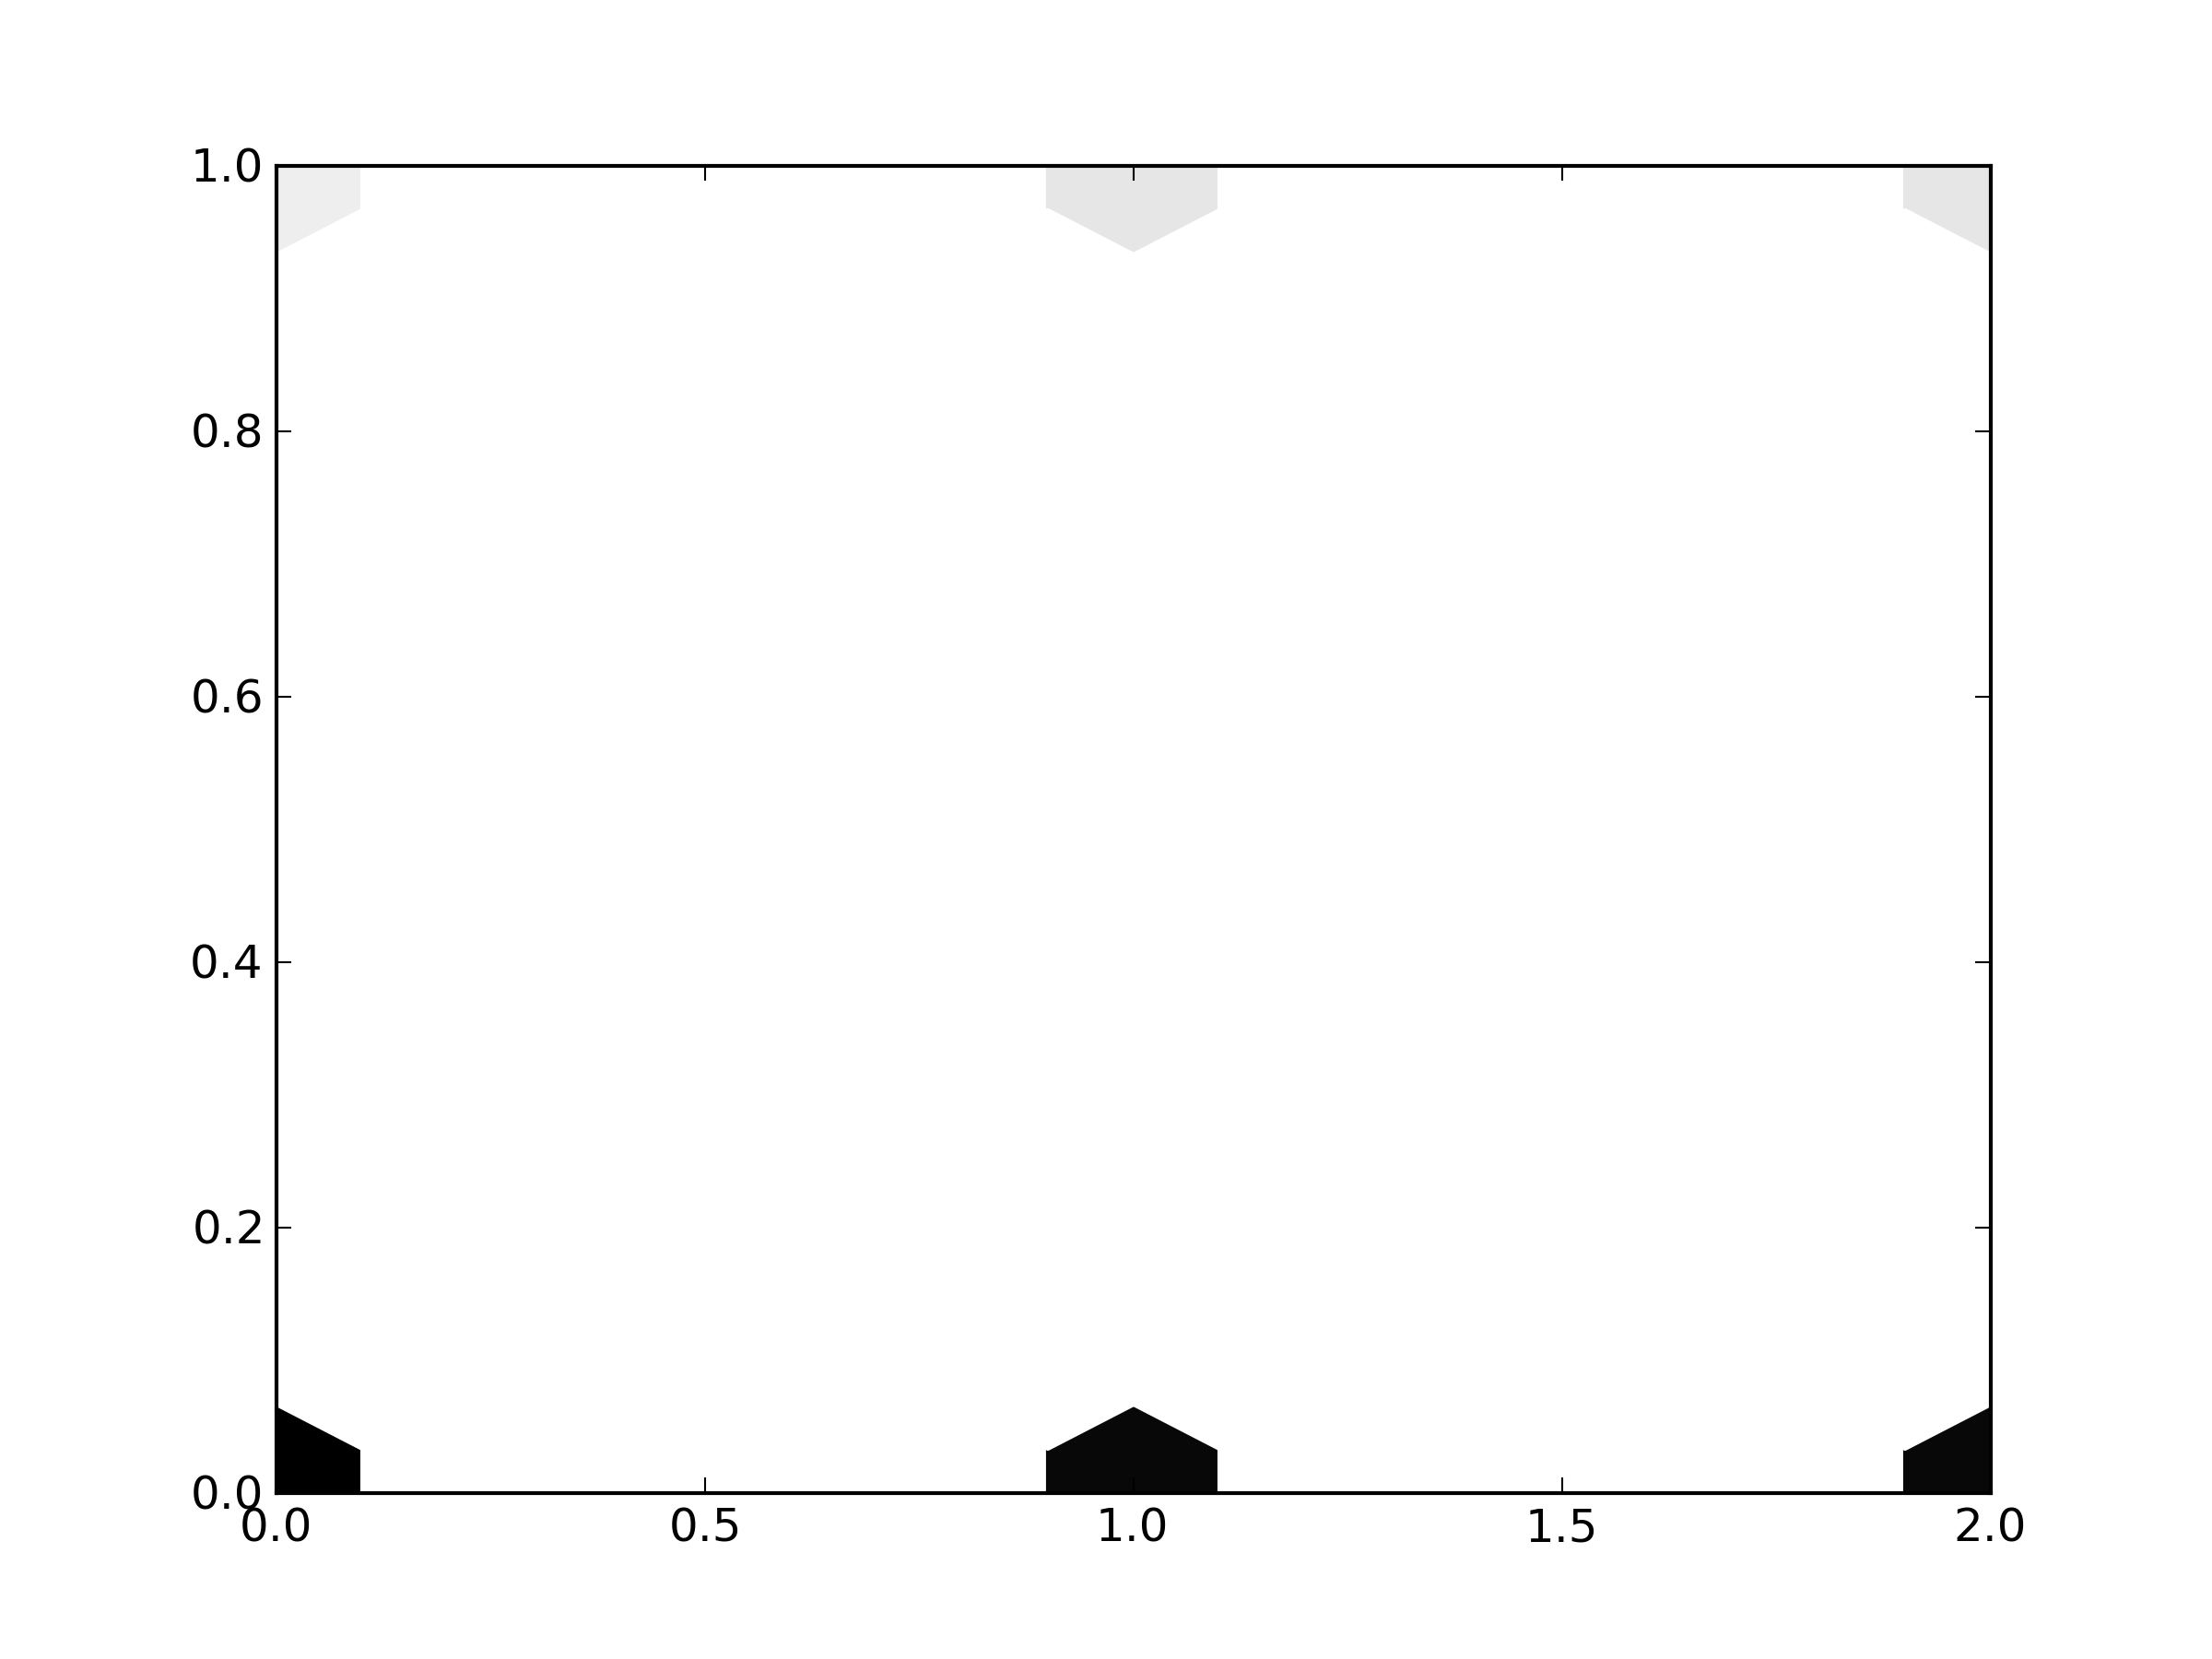
\includegraphics[width=\textwidth]{pop10iter.png}
\label{fig:pop10iter}
\end{figure}

\begin{figure}[h]
\caption{A histogram of proportion of cooperations per round after
  25,000 rounds with $N=20$ and $I \in \{10,20,50,100,200\}$.}

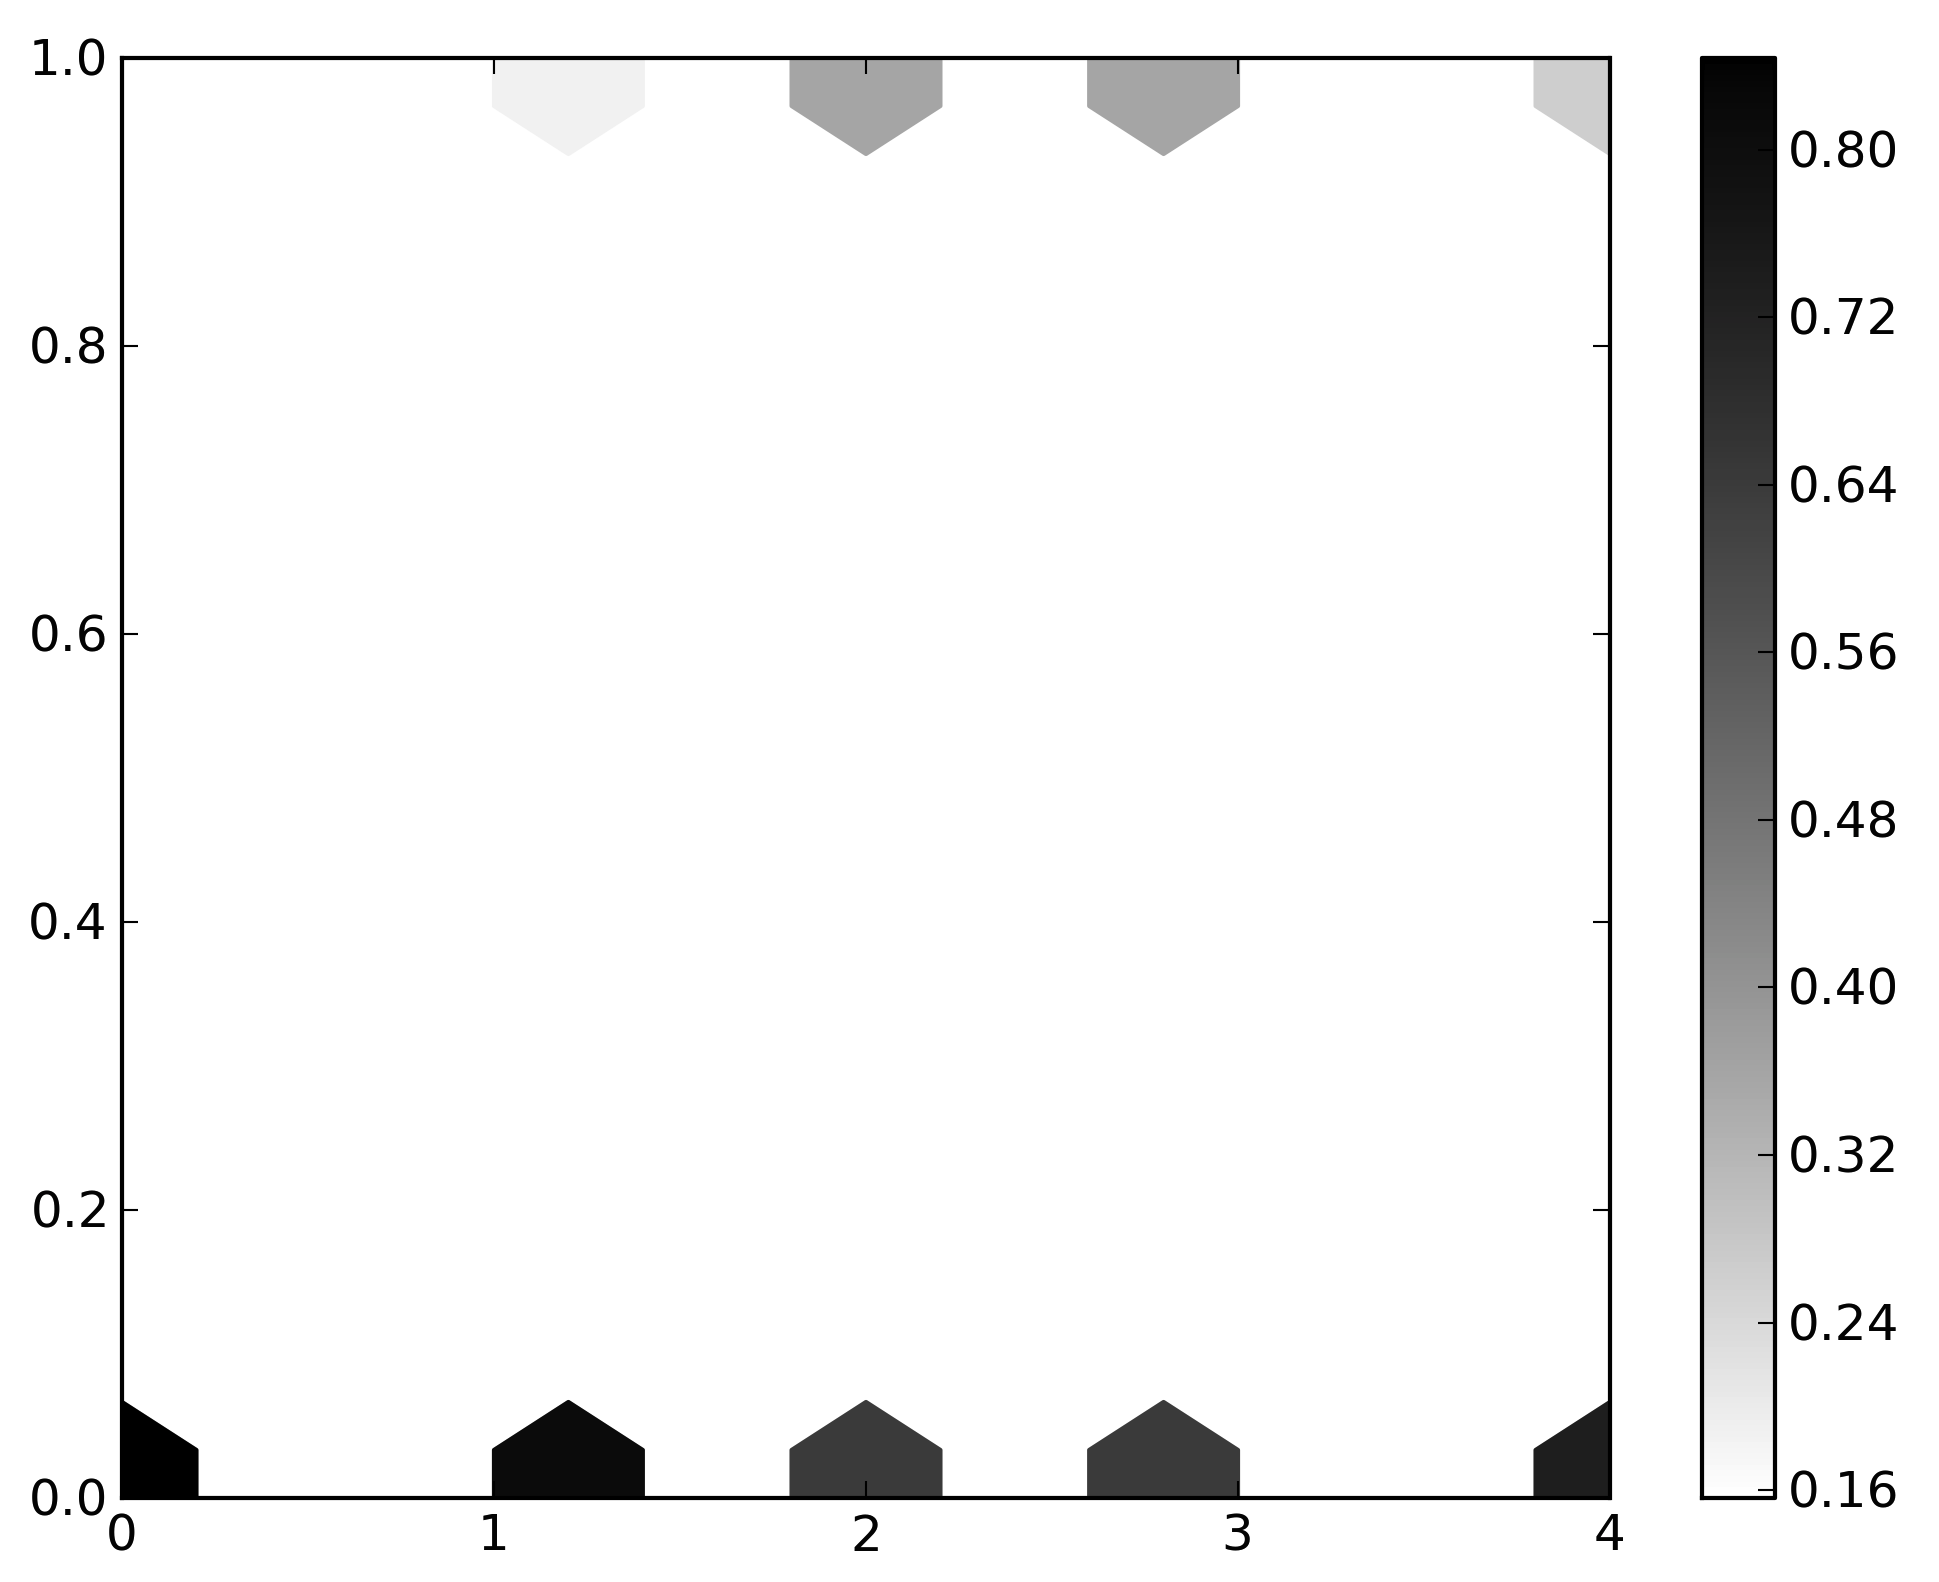
\includegraphics[width=\textwidth]{pop20iter.png}
\label{fig:pop20iter}
\end{figure}

\begin{figure}[h]
\caption{A histogram of proportion of cooperations per round after
  25,000 rounds with $N=50$ and $I \in \{10,20,50,100,200,500\}$.}

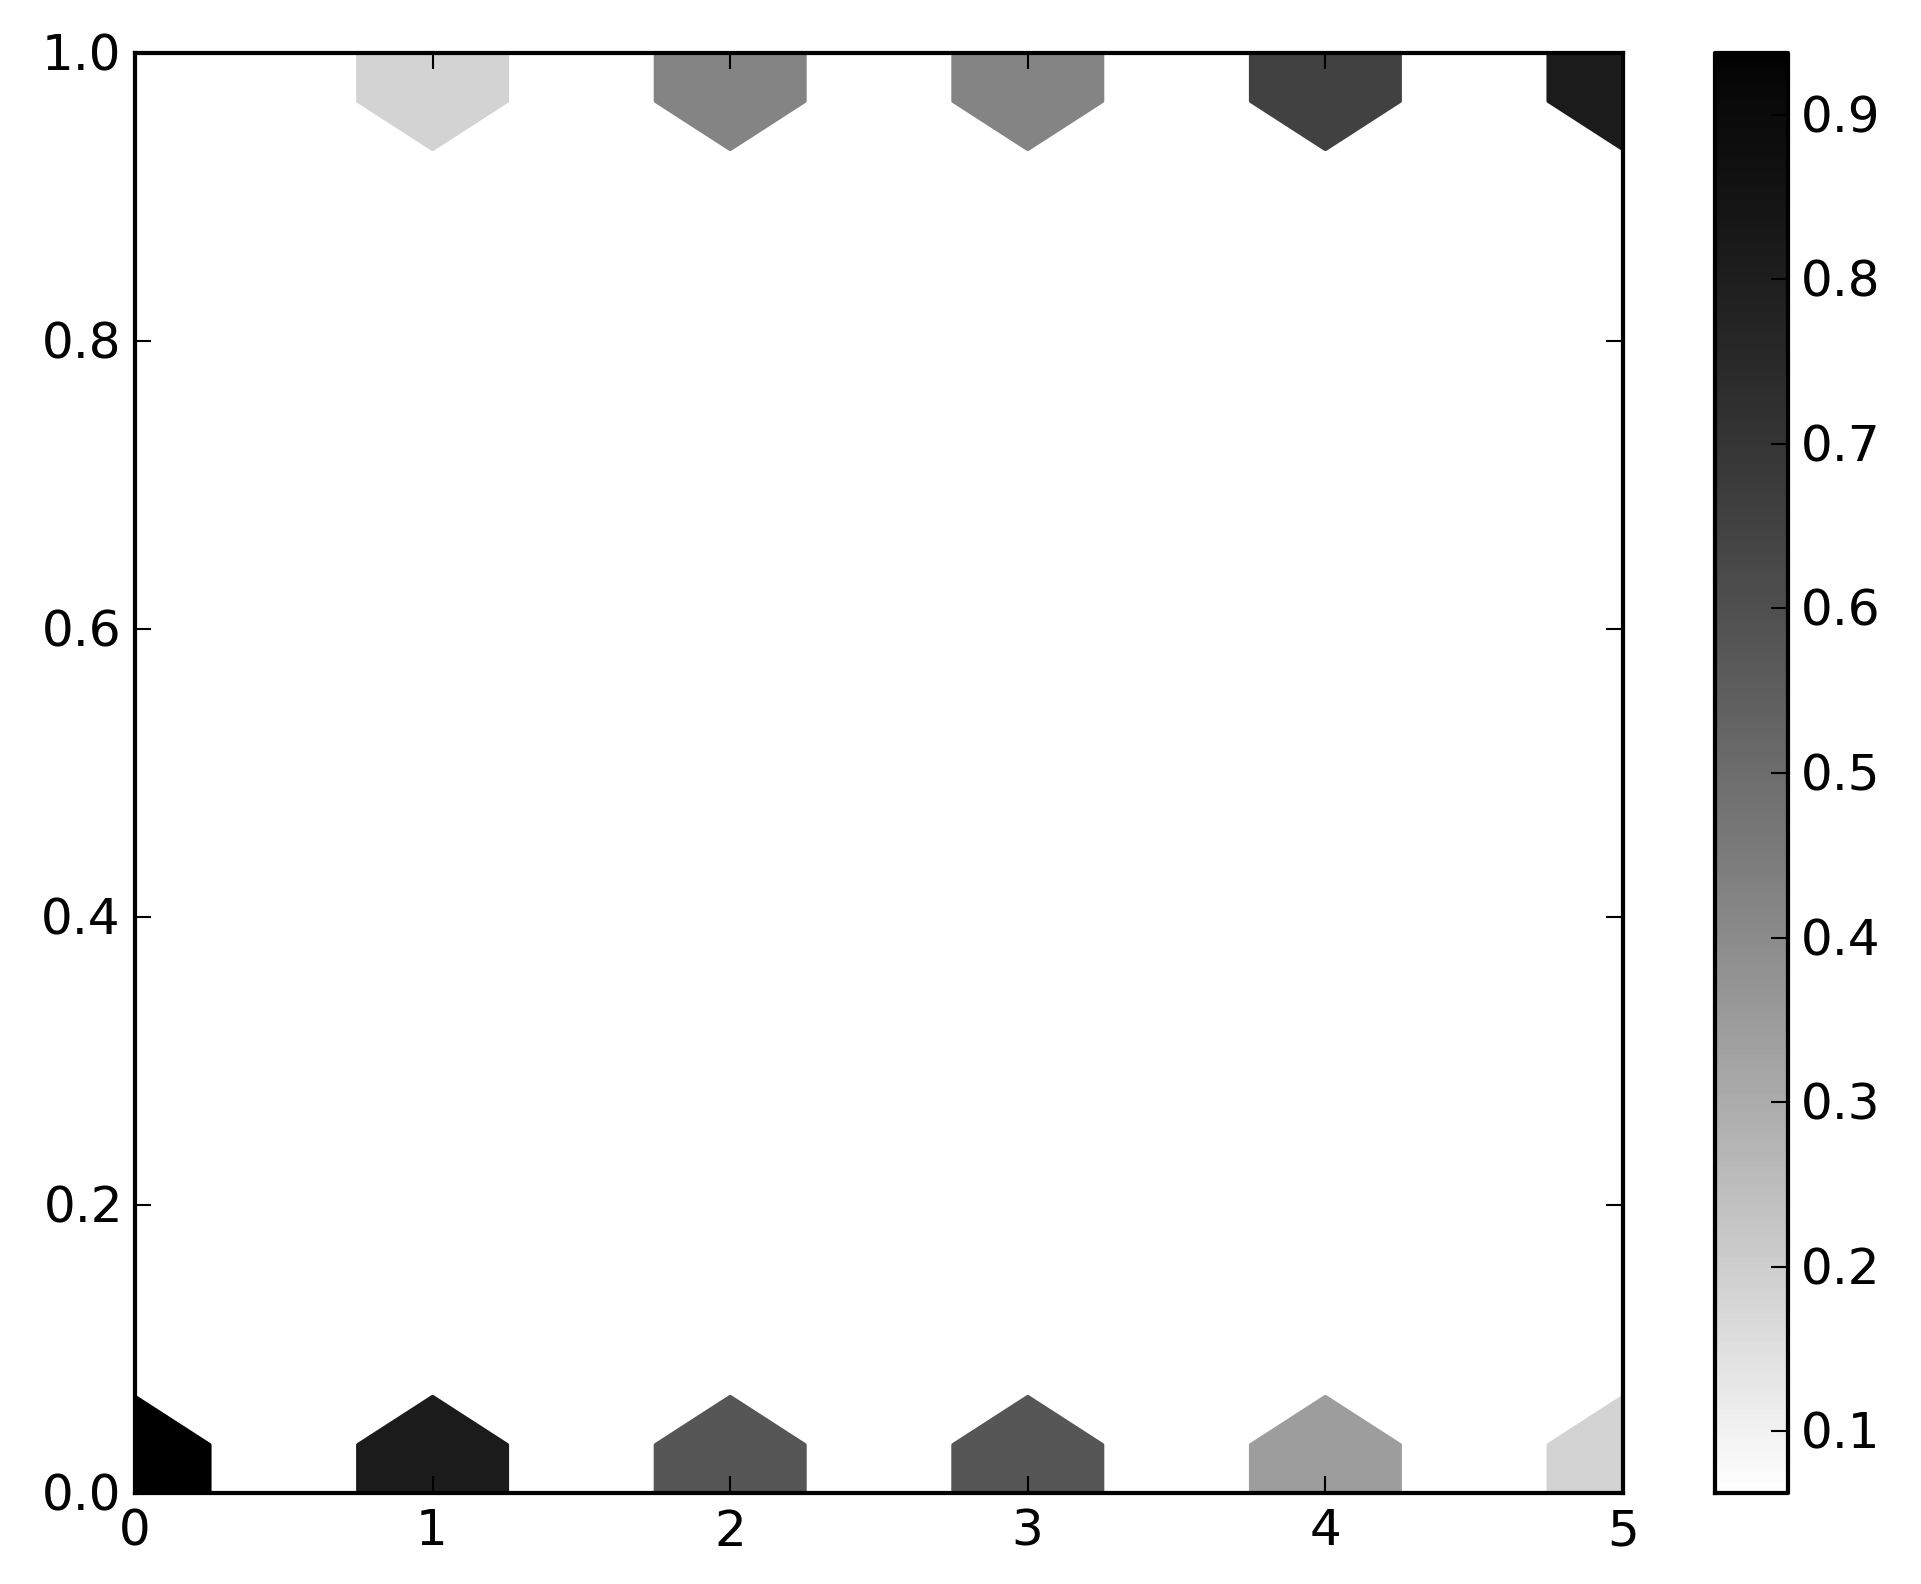
\includegraphics[width=\textwidth]{pop50iter.png}
\label{fig:pop50iter}
\end{figure}

\begin{figure}[h]
\caption{A histogram of proportion of cooperations per round after
  25,000 rounds with $N=100$ and $I \in \{10,20,50,100,200,500\}$.}

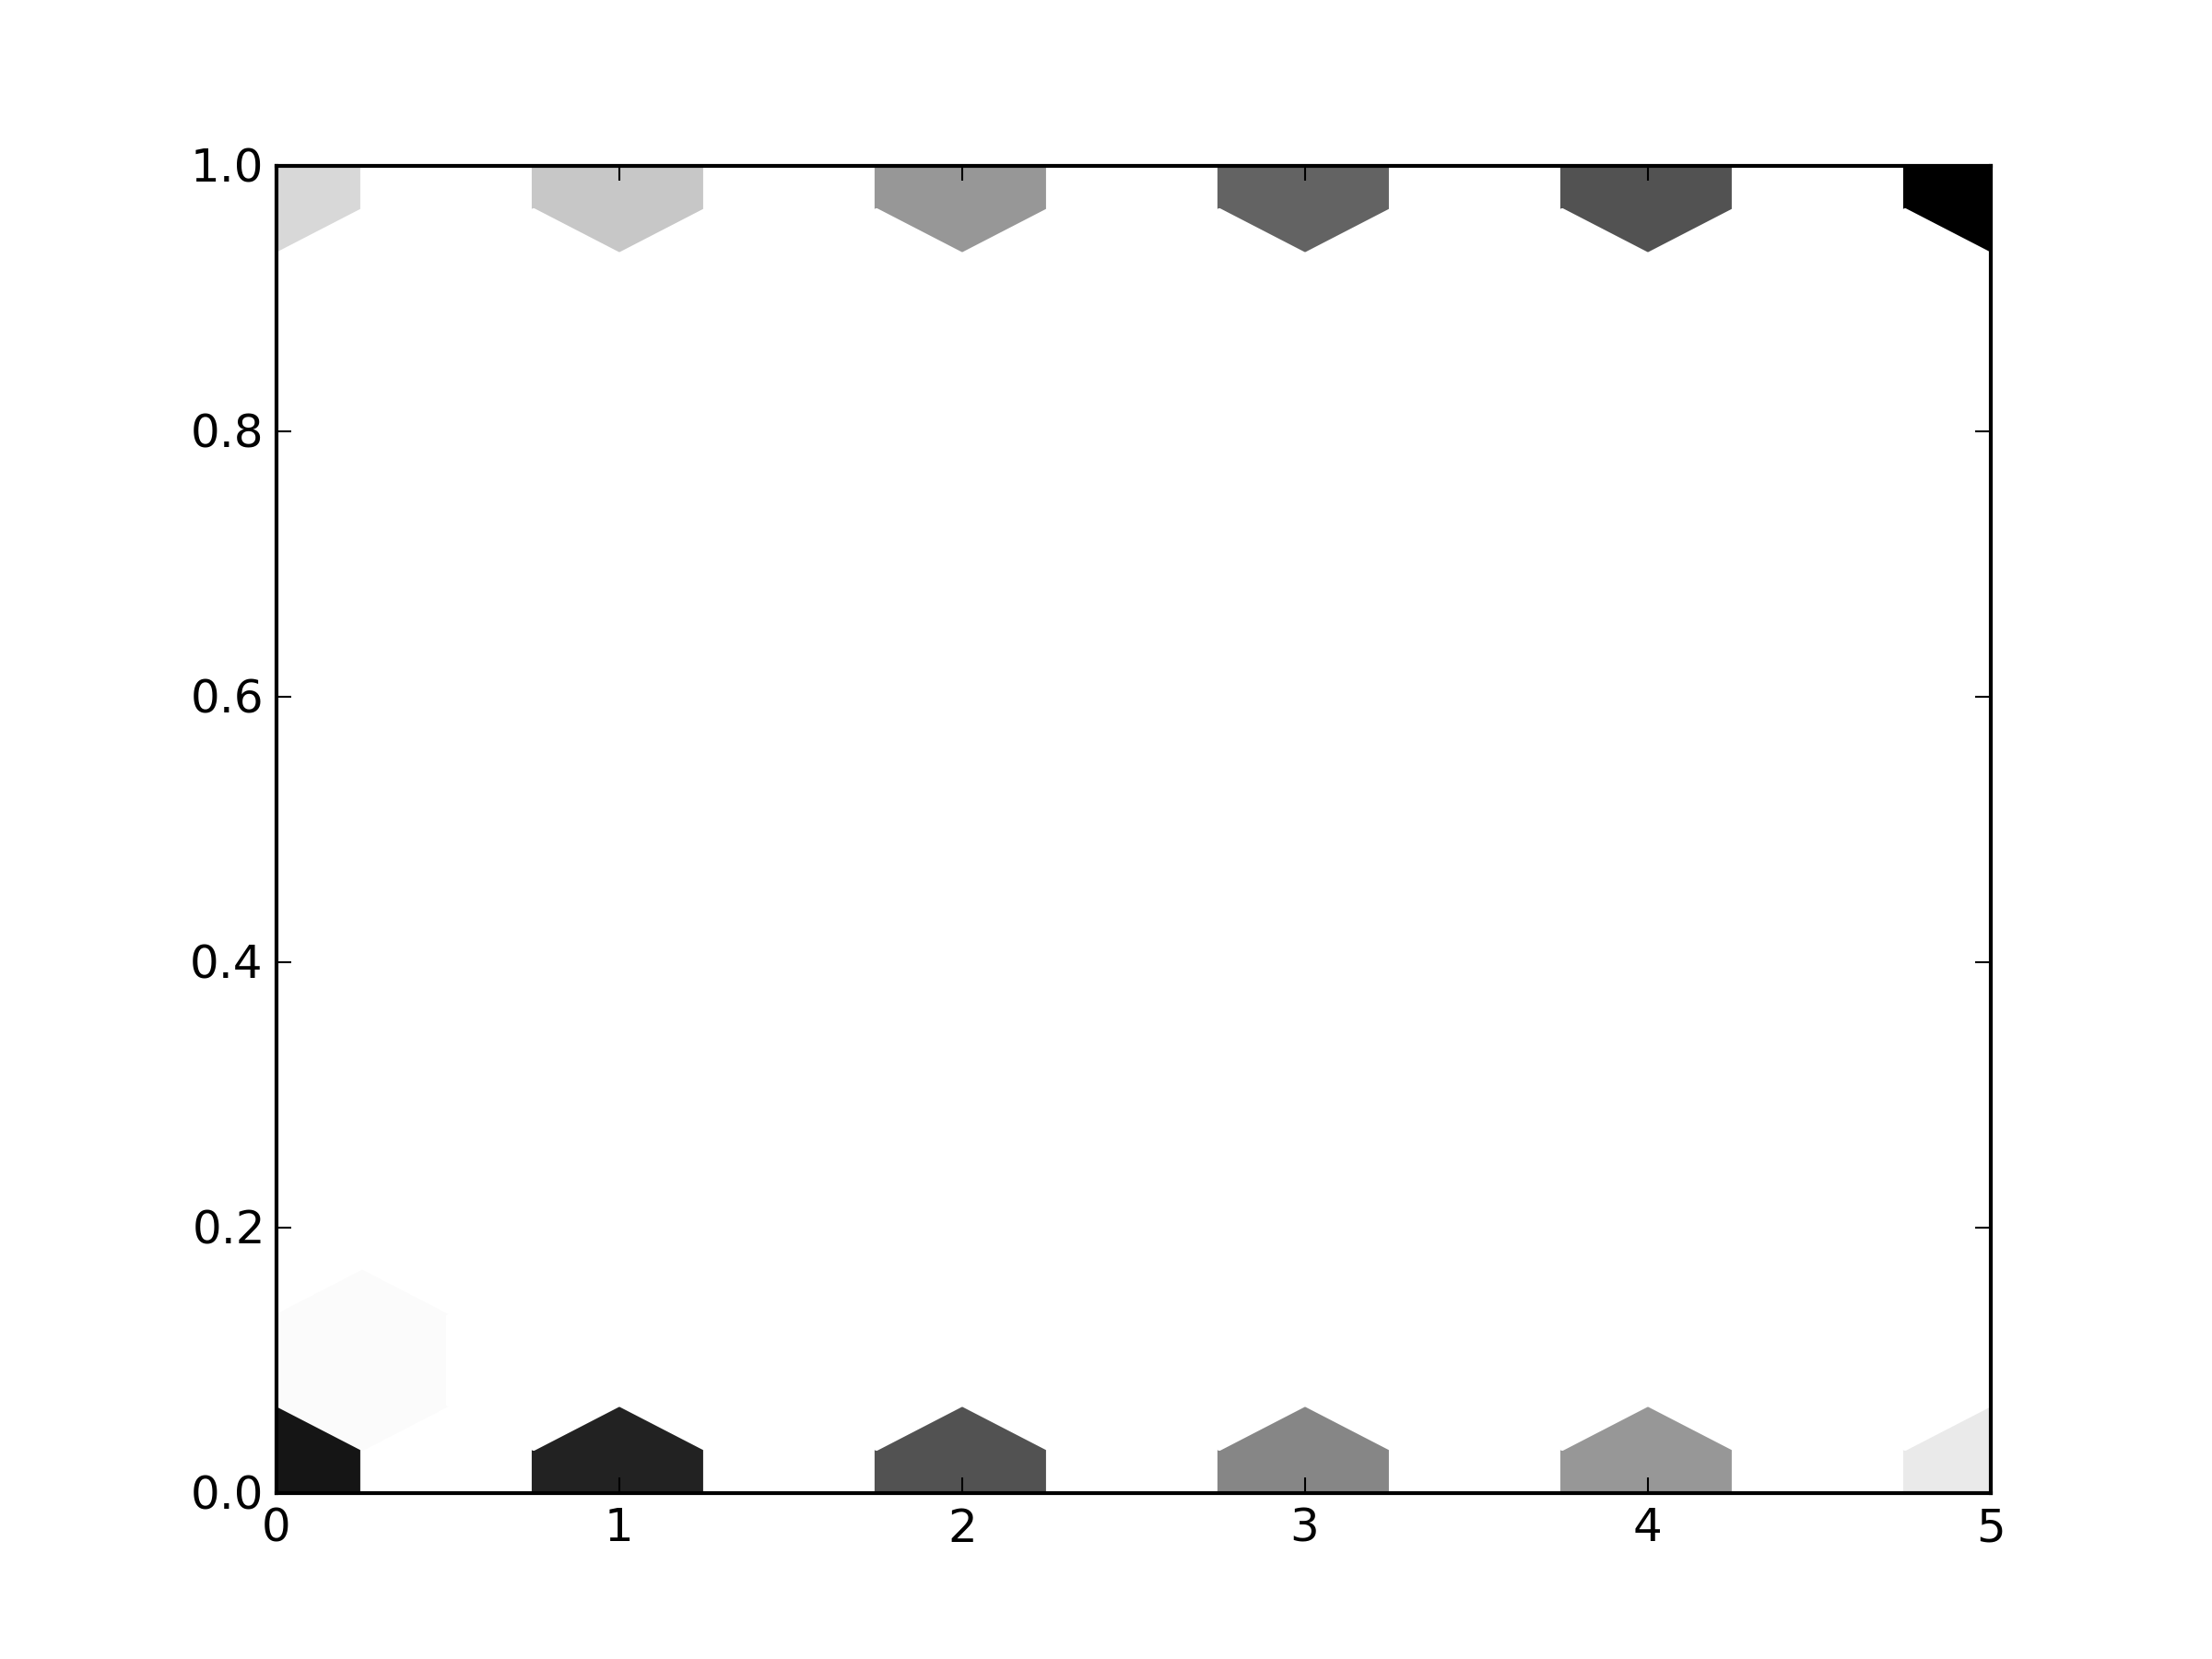
\includegraphics[width=\textwidth]{pop100iter.png}
\label{fig:pop100iter}
\end{figure}

\subsection{Dependence on population size}

In an extremely counter-intuitive twist, we found that larger
populations had a \emph{higher} probability of fixating at cooperation
with $I=N$. This implies that the number of interactions per round
required to have a probability $p$ of cooperation fixating grows
significantly \emph{sublinearly} with increasing population size
rather than linearly as our argument in section
\ref{sec:inter_per_round} suggests. We were unable to determine why
this surprising result holds and admit extreme bafflement.

\subsection{Long-range behavior}
\label{sec:longrange}
Over hundreds of thousands of rounds the typical behavior (with $b=2$,
$c = d = 0.05$, $N = I = 100$, $\omega = 0.1$, $\mu = 0.0001$) can be
seen in figures \ref{fig:really} and \ref{fig:what} below.

\begin{figure}[h]
\caption{$10^6$ rounds with the parameters listed in section
  \ref{sec:longrange}. Green trend lines are average reputation, blue
  are average strategy, and red are average fitness. Observe that in
  the first two runs, cooperation emerges even after a selfish
  strategy has fixated.}

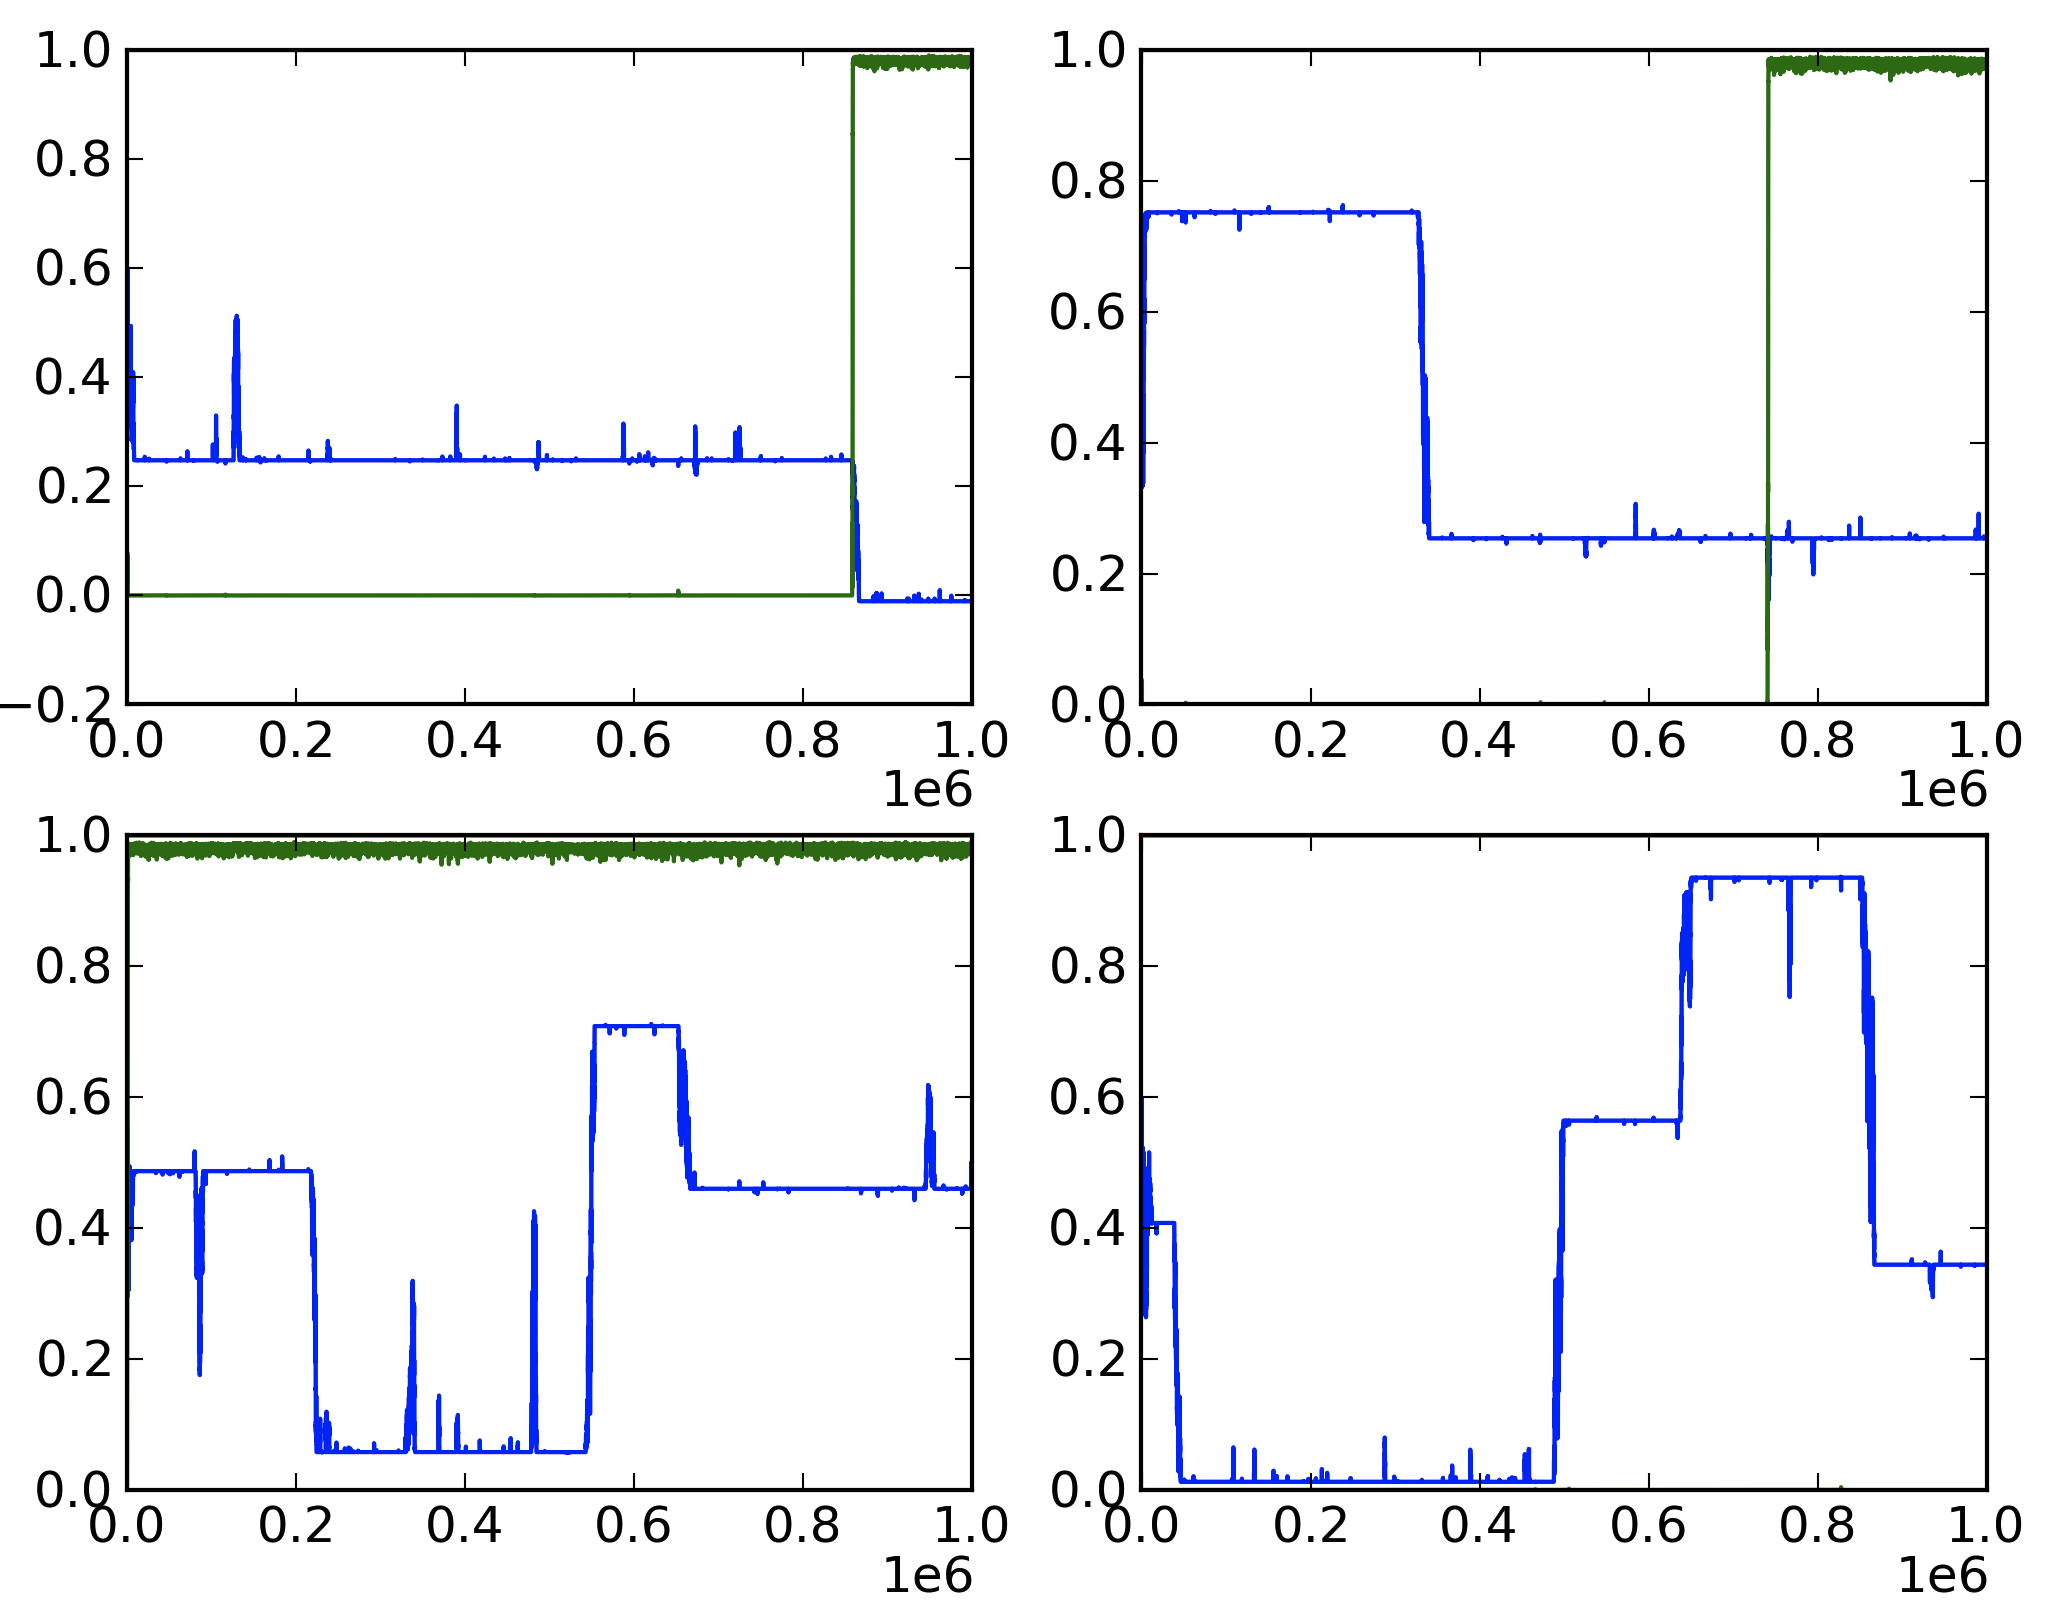
\includegraphics[width=\textwidth]{really.png}
\label{fig:really}
\end{figure}
\begin{figure}[h]
\caption{$2 \times 10^6$ rounds with the parameters listed in section
  \ref{sec:longrange}. Note how in the first run, cooperation is
  invaded by a high-threshold, selfish strategy.}

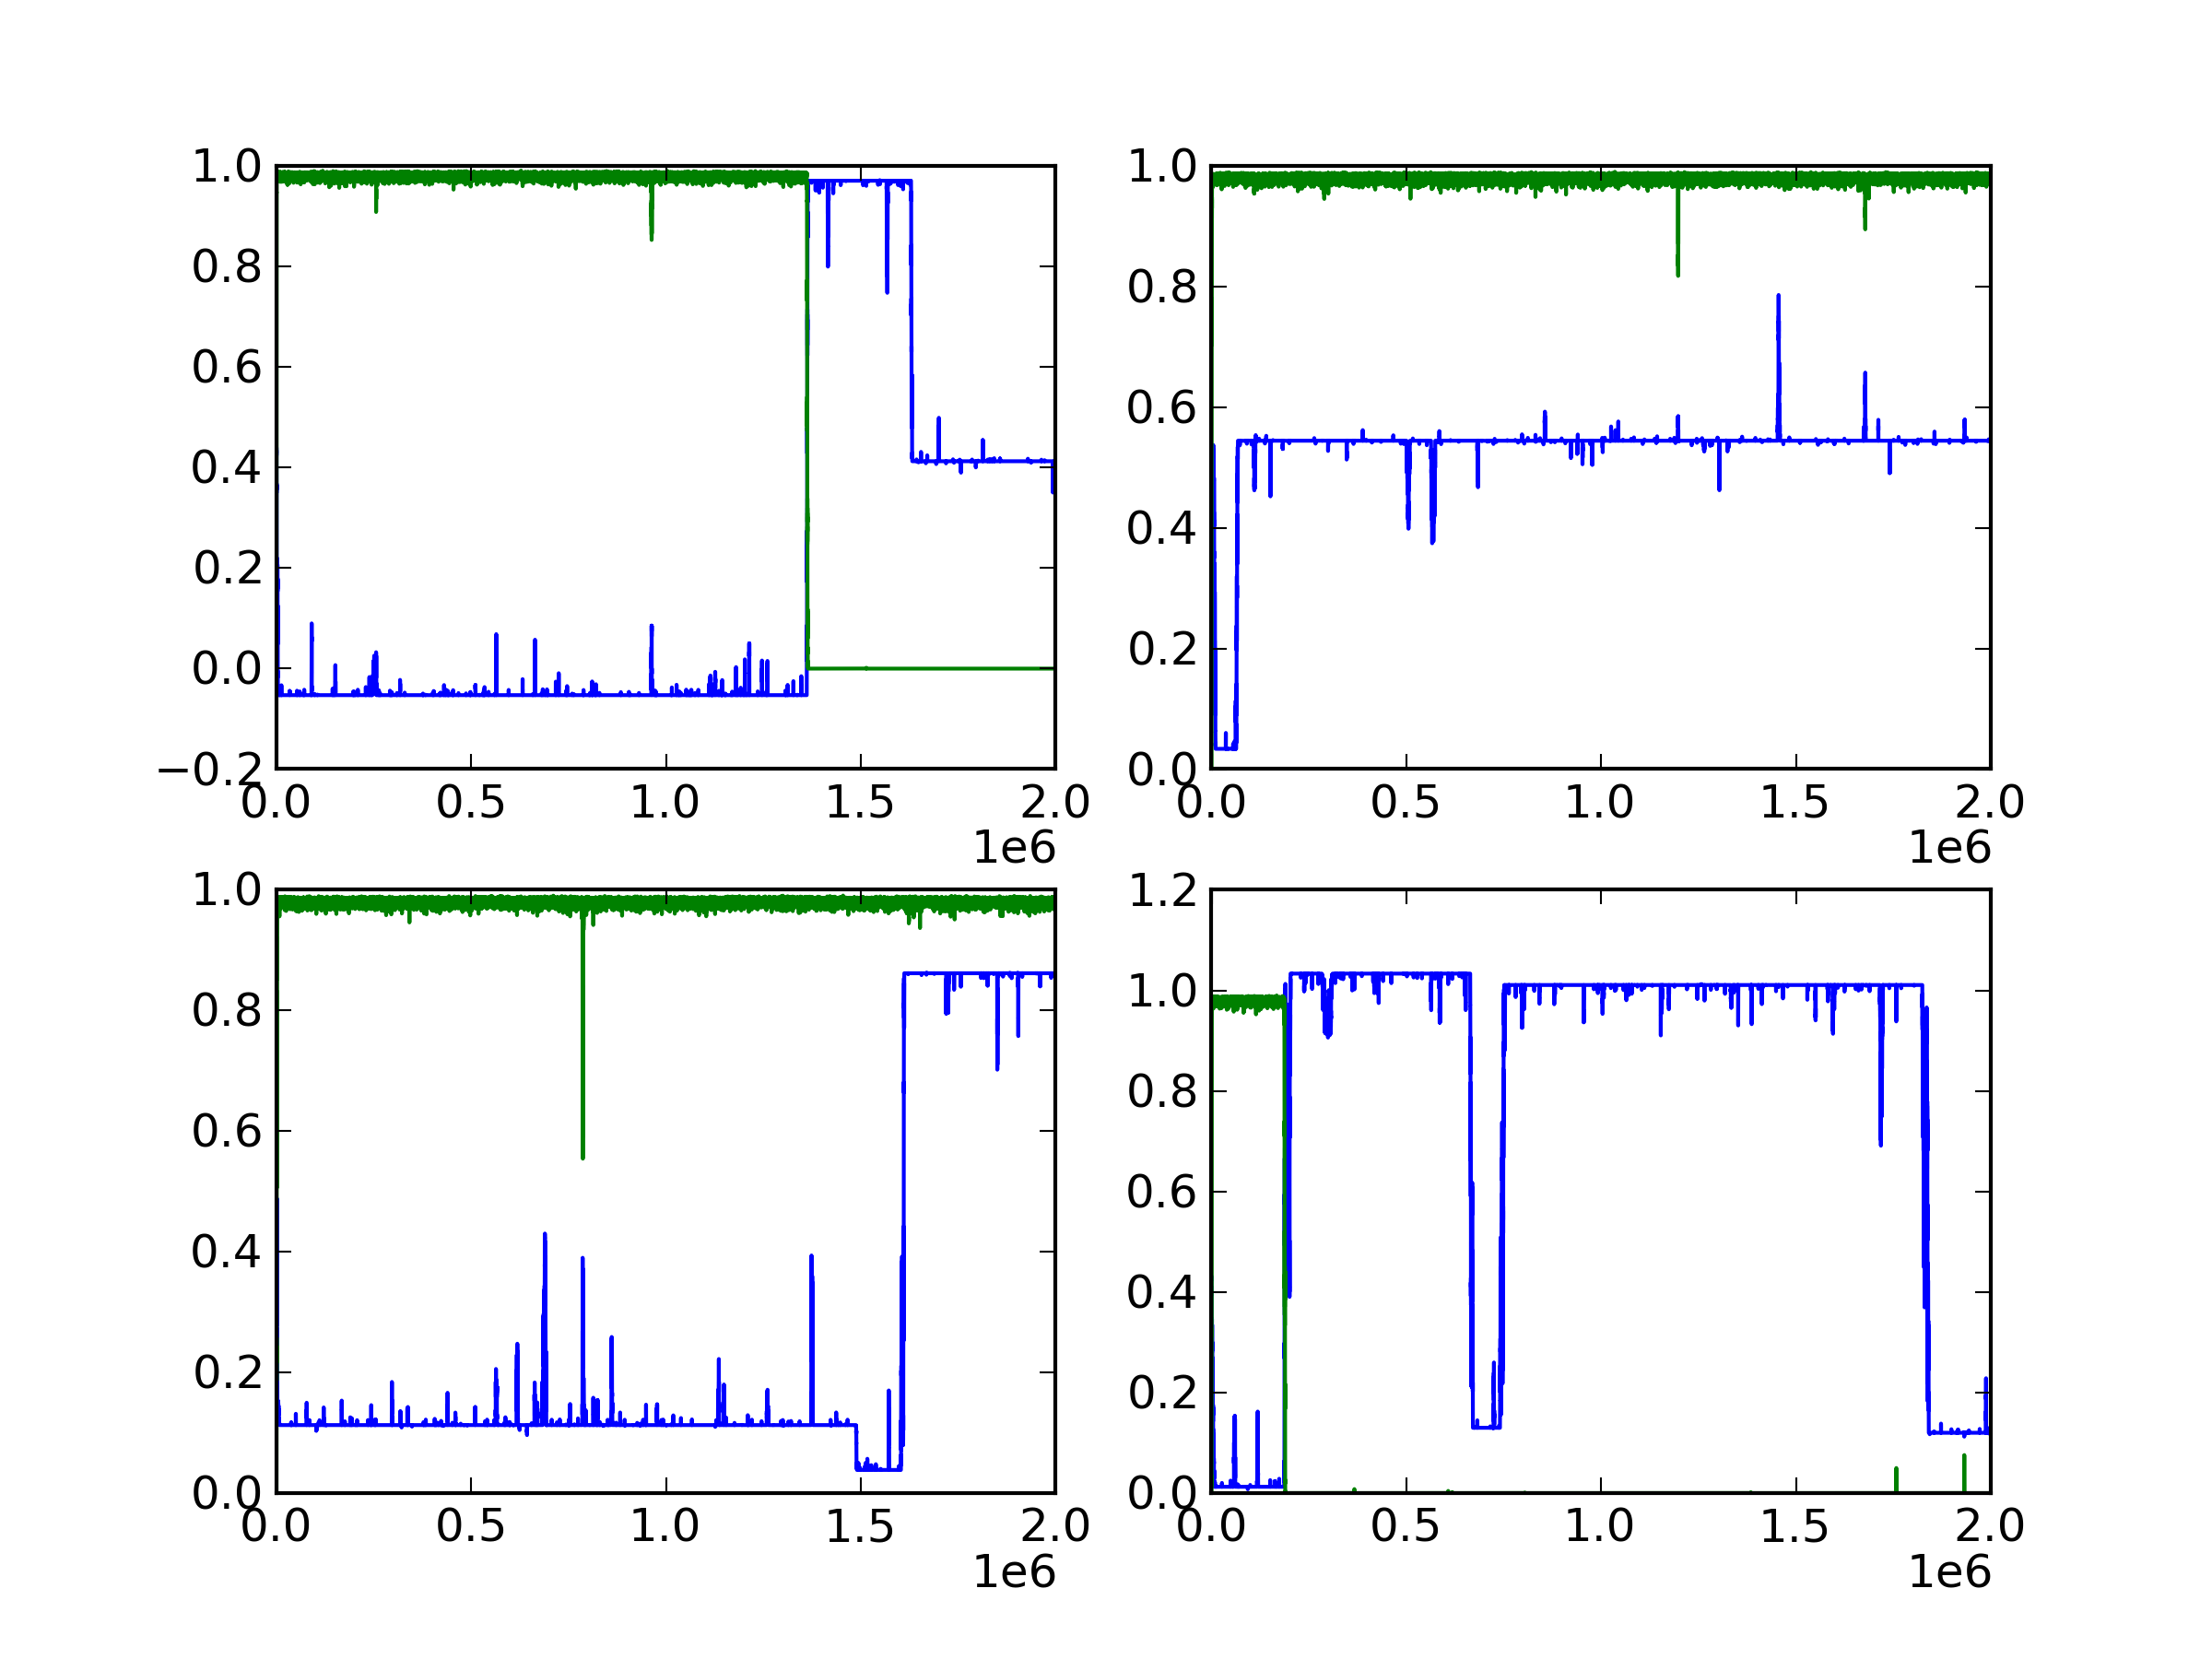
\includegraphics[width=\textwidth]{what.png}
\label{fig:what}
\end{figure}


This replicates Sigmund and Nowak's result
\cite{nowak_evolution_1998}, although with a much lower benefit/cost
ratio than used in that model. With each step taking many hundred
thousand time intervals, cooperation fixates after a critical mass of
cooperators kickstarts an increase in reputations, average strategy
falls below zero as everyone becomes an unconditional cooperator by
random drift, and finally unconditional defectors invade and take over
starting the cycle again. As is often seen for invasions by new types
in models like this, many of the transitions can fail the first times
they start to occur.

The first step is dependent on there being unconditional cooperators
and the last on there being unconditional defectors.


\section{Conclusion}
\label{sec:conclusion}

\section{Further directions}

\subsection{Analytic results}

Because of the nontrivial way in which past interactions affect the
current round, analytic results on this model are rather
difficult. However, mathematical bounds on PageRank obtained by
Bianchini et al. \cite{bianchini_Inside_2005} and Langville et
al. \cite{langville_deeper_2004} suggest that some theoretical results
may be possible.

\subsection{Computational constraints}

In reality, it is not free to compute a PageRank matrix with arbitrary
precision. It would be interesting to see if limiting the precision to
which the vector was calculated has any effect on how quickly or how
often cooperative strategies fixate in the population. In fact, this
could even be an additional feature subject to evolution and
mutation. With appropriate fitness costs for more precise calculation,
one might even be able to obtain theoretical validation for Dunbar's
number, the number of individuals beyond which social groups start to
break down \cite{dunbar_neocortex_1995}.

\bibliographystyle{plain} \bibliography{refs}

\end{document}
